\documentclass[11pt,a4paper]{article}

\usepackage[margin=2.4cm]{geometry}
\usepackage{lmodern}
\usepackage[T1]{fontenc}
\usepackage[utf8]{inputenc}
\usepackage{amsmath,amssymb,amsthm,bm}
\usepackage{booktabs,array}
\usepackage{microtype}
\usepackage{setspace}
\usepackage{xcolor}
\usepackage{caption}
\usepackage{placeins}
\usepackage{tikz}
\usetikzlibrary{arrows.meta,positioning}
\usepackage[hidelinks]{hyperref}

\definecolor{ltink}{HTML}{1B4F72}
\definecolor{ltsoft}{HTML}{EAF0F4}
\hypersetup{colorlinks=true,linkcolor=ltink,citecolor=ltink,urlcolor=ltink}

\newcommand{\E}{\mathbb{E}}
\newcommand{\Var}{\mathrm{Var}}
\newcommand{\Cov}{\mathrm{Cov}}
\newcommand{\Corr}{\mathrm{Corr}}
\newcommand{\h}{h^{2}}
\newcommand{\ind}{\perp\!\!\!\perp}
\newcommand{\doi}[1]{doi:\allowbreak\texttt{#1}}

\title{%
  \vspace{-1.4em}
  {\large Notes}\\[0.4em]
  {\LARGE\bfseries Posterior mean genetic liability\\[0.15em]
  from family history}\\[0.55em]
  {\large Model, sequential approximation, and evidence in \texttt{ltpred}}}
\author{Bjarni J\'ohann Vilhj\'almsson\\[0.35em]
  {\small\texttt{https://github.com/bvilhjal/ltpred}\quad$\cdot$\quad v0.3.0}}
\date{13 August 2026}

\begin{document}
\maketitle
\thispagestyle{plain}

\begin{abstract}
\noindent
The LT-FH family of methods replaces a case/control label with
$\E[a_i\mid \text{family data}]$ under a Gaussian liability-threshold
model. That is ordinary BLUP after the liabilities have been replaced
by their truncated-normal means; the published names
(LT-FH, LT-FH++, ADuLT, PA-FGRS) are different choices of the
truncation region \(C_F\), not different genetic models.
These notes fix the estimand, the observation-model menu, the
exactness boundary of the Pearson--Aitken (PA) approximation, and
the sampling conditions under which a pedigree Haseman--Elston
fit recovers \(\h\).
Simulation under the model's own generative assumptions gives
$\Corr(\mathrm{PA},\mathrm{Gibbs})\ge 0.9977$ without the censoring
mixture, a classic-LT-FH causal-SNP noncentrality ratio of
$1.47\pm 0.04\times$ over case/control (independent SNPs), and a
paired $+0.145\pm 0.015$ LT-FH++ increment over matched ADuLT when
onset is a deterministic function of liability and the CIP is known.
Those last two figures are upper bounds relative to register data.
They are not estimates of clinical utility.
\end{abstract}

\vspace{0.4em}
\noindent
The intended reader already uses GWAS, liability-scale \(\h\), and
Falconer's threshold construction. The notes do not re-derive those.
They are about what is being conditioned on, where the sequential
approximation is exact, and which simulation claims survive their
generative assumptions.

%----------------------------------------------------------------------
\section{Estimand}
\label{sec:estimand}

Write $a_i$ for the additive genetic liability of a designated
proband, $\Var(a_i)=\h$ on the usual unit-liability scale, and
$\ell_F$ for the vector of full liabilities on the people whose
disease records are used (the proband may or may not be among them).
The data determine a rectangle $C_F$---one interval per person---and
the target is
\begin{equation}
  \mu_i
  \;=\;
  \E\!\bigl[a_i \,\big|\, \ell_F\in C_F,\; A,\; \h,\; K(\,\cdot\,)\bigr],
  \label{eq:estimand}
\end{equation}
where $A$ is the additive relationship matrix and $K(\,\cdot\,)$ is
the prevalence or cumulative-incidence model that turns status and
age into interval endpoints.

If $\ell_F$ were observed continuously, \eqref{eq:estimand} would be
the selection index / animal-model BLUP
\begin{equation}
  \E[a_i\mid \ell_F]
  \;=\;
  \Cov(a_i,\ell_F)\,\Var(\ell_F)^{-1}\,\ell_F
  \label{eq:blup}
\end{equation}
\cite{hazel1943,henderson1975}.
A single relative with relationship $r$ contributes $r\,\h\,\ell_r$.
Disease records do not give $\ell_F$. They give
$\ell_F\in C_F$. Under joint normality,
\begin{equation}
  \E[a_i\mid \ell_F\in C_F]
  \;=\;
  \Cov(a_i,\ell_F)\,\Var(\ell_F)^{-1}\,
  \E[\ell_F\mid \ell_F\in C_F].
  \label{eq:blup-trunc}
\end{equation}
The BLUP weights are unchanged; only the right-hand side is replaced
by a truncated-normal mean.
The map from the binary (or censored) records to $\mu_i$ is therefore
nonlinear, and reduces to \eqref{eq:blup} only when every interval
collapses to a point.

Two immediate consequences, both easy to get wrong in an analysis.

\begin{enumerate}
\item \textbf{The proband's own diagnosis is optional.}
  Include it when $\mu_i$ is a GWAS phenotype \emph{constructed from}
  that diagnosis \cite{hujoel2020,pedersen2022}.
  Leave the corresponding interval as $(-\infty,\infty)$ when the
  same diagnosis is the outcome you will later predict or classify.
  Conditioning on the answer is leakage, not sophistication.
\item \textbf{\eqref{eq:estimand} is not a SNP polygenic score.}
  No marker effects enter.
  Combining $\mu_i$ with a PGS is a downstream model
  \cite{hujoel2022,krebs2026}.
\end{enumerate}

The multivariate threshold model on a pedigree is Sham's
framework \cite{sham1998}.
So, Kwan, Cherny and Sham \cite{so2011} already combined family
history with known loci, age, and competing mortality; they targeted
absolute risk.
Here the target is the breeding value, used as a phenotype.

\begin{figure}[ht]
\centering
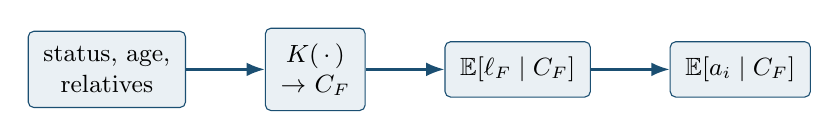
\begin{tikzpicture}[
  font=\small,
  box/.style={draw=ltink, rounded corners=2pt, align=center,
              inner sep=5.5pt, fill=ltsoft},
  arr/.style={-{Latex}, ltink, thick}
]
  \node[box] (data) {status, age,\\relatives};
  \node[box, right=10mm of data] (thr) {$K(\,\cdot\,)$\\$\to$ $C_F$};
  \node[box, right=10mm of thr] (tmvn) {$\E[\ell_F\mid C_F]$};
  \node[box, right=10mm of tmvn] (blup) {$\E[a_i\mid C_F]$};
  \draw[arr] (data) -- (thr);
  \draw[arr] (thr) -- (tmvn);
  \draw[arr] (tmvn) -- (blup);
\end{tikzpicture}
\caption{The published methods differ in how they build $C_F$.
They share \eqref{eq:blup-trunc}.}
\label{fig:pipeline}
\end{figure}

%----------------------------------------------------------------------
\section{Covariance}
\label{sec:ltm}

The liability split is the usual one,
\begin{equation}
  \ell = a + e,
  \qquad
  a\sim\mathcal{N}(0,\h),\quad
  e\sim\mathcal{N}(0,1-\h),\quad
  a\ind e,
\end{equation}
so $\ell\sim\mathcal{N}(0,1)$ and a case is $\ell>T$ with
$T=\Phi^{-1}(1-K)$ at a single prevalence $K$
\cite{wright1934,falconer1965}.
On a pedigree,
\begin{equation}
  \Cov(a_i,a_j)=\h A_{ij},
  \qquad
  \Cov(\ell_i,\ell_j)=\h A_{ij}\ (i\neq j),
  \qquad
  \Var(\ell_i)=1,
  \label{eq:animal}
\end{equation}
with $A_{ij}=2\phi_{ij}$.
Mates are taken as unrelated ($A_{mf}=0$): the default $A$ is not a
generative model of assortment.
Inbreeding is handled by the tabular method \cite{henderson1976},
after which full liabilities are rescaled to unit variance so that
$\Phi^{-1}(1-K)$ still means prevalence $K$.

Shared environment is optional and off-diagonal,
\begin{equation}
  \Cov(\ell_i,\ell_j)
  \;=\;
  \h A_{ij} + c^{2} C_{ij} + m^{2} M_{ij},
  \qquad \h+c^{2}+m^{2}\le 1.
  \label{eq:ACE}
\end{equation}
The target $a_i$ still couples to relatives only through $\h A$.
Identification is the usual contrast arithmetic: $C$ (full-sib
environment) is the excess of sib covariance over parent--offspring
(both have $A=\tfrac12$); $M$ (couple) is the covariance of
genetically unrelated mates, and therefore confounds household
sharing with assortment \cite{robinson2017}.
A directional maternal effect is not a symmetric kernel and is not
$M$.
An environment that scales with $A$ is absorbed into $\h$ and is
not estimable.
Nuclear families give roughly three contrasts; a bank of
relationship-specific environments needs the relative types that
extended pedigrees supply.
This is the pedigree analogue of why ACE is identified from MZ/DZ
twins and $A+C+D$ is not.

One inherited LTFHPlus convention is worth knowing before comparing
constructors: two same-side half-sibs in the role grammar are
related $\tfrac12\h$ \emph{to each other} (implied shared second
parent).
A pedigree in which they have distinct other parents must be built
from $A$, not from those role labels.

%----------------------------------------------------------------------
\section{The observation-model menu}
\label{sec:obs}

LT-FH, LT-FH++ and ADuLT are names for $C_F$, not for an inference
algorithm.
Gibbs and PA both apply to the first three.
PA-FGRS, in the published specification and in the implementation,
is PA-specific.

\paragraph{Classic LT-FH \cite{hujoel2020}.}
One $K$, one $T$.
Cases $[T,\infty)$, controls $(-\infty,T]$, relatives included.
This is the configuration-specific successor of GWAX \cite{liu2017}.

\paragraph{LT-FH++ and ADuLT \cite{pedersen2022,pedersen2023}.}
Age, sex and cohort enter only through a CIP $K(t;s,b)$ and
\begin{equation}
  T_i \;=\; \Phi^{-1}\!\bigl(1-K(t_i;s_i,b_i)\bigr).
\end{equation}
A control at current age $c_i$ is truncated above at $T_i(c_i)$.
A case with onset $a_i$ is \emph{pinned} at $T_i(a_i)$ (lower $=$
upper).
The same $T_i$ with relatives is LT-FH++; without them, ADuLT.

Pinning is the strong assumption in this construction, and it is
easy to understate.
It says that the CIP is an error-free map from liability to onset,
that onset dates are exact, and that two cases with the same
stratum and onset have identical liability---zero residual variance
given $a_i$.
The inverse map is then the identity: the observation \emph{is}
the liability.
When onset is a window, or $K$ is estimated, an interval
$[T_i(a_i),\infty)$ or the lifetime interval $[T_{\mathrm{pop}},\infty)$
is the more honest likelihood.

Because the BLUP weights in \eqref{eq:blup-trunc} do not depend on
the $T_i$, a shared threshold error is mostly a calibration shift.
A stratum-specific error also reorders scores.

\paragraph{Base PA-FGRS \cite{krebs2024}.}
Observed cases use the \emph{lifetime} interval
$[\Phi^{-1}(1-K_{\mathrm{pop}}),\infty)$.
Age enters for censored controls through the mixture in
Section~\ref{sec:mixture}, not through the case threshold.
Helpers that put cases above $T_i(a_i)$ are a different observation
model; they are not PA-FGRS$_{\mathrm{ADT}}$.
Kendler's FGRS \cite{kendler2021} is a third thing and is not
implemented.

\paragraph{PGS and $\mu_i$.}
Split $a=s+u$ with $\Var(s)=p:=\h_{\mathrm{SNP}}/\h$.
If two standardised scores satisfy
$\mathrm{PGS}\ind\mu\mid a$, then
\begin{equation}
  \Corr(\mathrm{PGS},\mu)
  \;=\;
  a_{\mathrm{PGS}}\,b_{\mu}\,\sqrt{p}
  \;=\;
  \sqrt{R^{2}_{\mathrm{PGS}}\,R^{2}_{\mu}\,p}.
  \label{eq:pgs-fh}
\end{equation}
The scores can each be genuinely predictive of $a$ and still almost
uncorrelated, because each is mostly noise relative to $a$
\cite{hujoel2022,krebs2026}.
Non-overlapping discovery and family samples remove one shared
noise term.
They do not imply the residual is zero (ancestry, assortment,
indirect effects, selection).

%----------------------------------------------------------------------
\section{Computing the truncated mean}
\label{sec:engines}

There is no closed form for $\E[\ell_F\mid C_F]$ once several
intervals are live.
Two approximations are used.

\subsection{Gibbs}

Coordinate-wise inverse-CDF sampling of the conditional
normals \cite{kotecha1999}, with coefficients from the precision
$Q=\Sigma^{-1}$:
$\mathrm{sd}_j=\sqrt{1/Q_{jj}}$,
$P_{ij}=-Q_{ij}/Q_{jj}$.
Pinned coordinates are held.
Far-tail intervals cannot be drawn on the probability scale
($\Phi$ underflows near $|z|\approx 38.5$); those use a log-scale
Rayleigh construction.
$\Sigma$ must be strictly positive definite.

The Monte Carlo standard error is the batch-means estimator
\cite{jones2006} that LTFHPlus takes from \texttt{batchmeans}.
Families that share a structure share one factorisation of
$\Sigma$; the rest is embarrassingly parallel.
This is the sampling-based reference for every no-mixture claim
below.

\subsection{Pearson--Aitken}
\label{sec:pa}

If one coordinate of a multivariate normal is selected from
$\mathcal{N}(m_i,v_i)$ to $(m^\star,v^\star)$, the others update by
\cite{pearson1903,aitken1935}
\begin{equation}
  m_j \leftarrow m_j+\frac{\Sigma_{ji}}{v_i}(m^\star-m_i),
  \qquad
  \Sigma_{jk} \leftarrow
  \Sigma_{jk}+\frac{\Sigma_{ji}\Sigma_{ik}}{v_i^{2}}(v^\star-v_i).
  \label{eq:pa}
\end{equation}
Mendell and Elston applied this sequentially to threshold traits
\cite{mendell1974}.
The implementation folds observed members last-to-first, then
applies the target's own interval to the updated
$\mathcal{N}(m_0,v_0)$.
For the genetic target the last step is a no-op
(bounds $(-\infty,\infty)$).
For $\E[\ell_o\mid C_F]$ it is the same estimand Gibbs uses.

After one truncation the selected law is no longer Gaussian.
PA keeps the first two moments and proceeds as if it were.
Hence: exact for a single interval or a pin; a sequential
two-moment approximation thereafter.
Fold order changes the error.
Canonicalising to a sorted role set makes the result a function of
the pedigree shape, not of input row order---reproducibility, not
accuracy.

On the no-mixture structures we have tested, that approximation
error is small enough to ignore for the posterior \emph{mean}
(Section~\ref{sec:results}).
It has not been characterised for the mixture, and PA's reported
conditional variance is itself an approximation.
A PA standard error of zero means no Monte Carlo error.

\subsection{Censored-control mixture}
\label{sec:mixture}

A person unaffected only up to current follow-up is a mixture of a
lifetime control and a not-yet-onset future case \cite{krebs2024}.
With current CIP $K_i$ and lifetime $K_{\mathrm{pop}}$,
\begin{equation}
  \pi
  \;=\;
  \frac{\Phi_{\mathrm{below}}}
       {\Phi_{\mathrm{below}}+(1-\Phi_{\mathrm{below}})
        (K_{\mathrm{pop}}-K_i)/K_{\mathrm{pop}}},
  \label{eq:mix}
\end{equation}
where the split is the \emph{lifetime} threshold and
$\Phi_{\mathrm{below}}$ is the current conditional mass below it.
The selected moments are the corresponding two-component mean and
variance.
Age enters only through $K_i$.

The factor $(K_{\mathrm{pop}}-K_i)/K_{\mathrm{pop}}$ is the CIP
probability that a future case has not yet onset.
That is an onset-timing assumption: among people who will
eventually be cases, time-to-onset is independent of liability,
and censoring is non-informative given the stratum.
If higher liability advances onset, the not-yet-onset component is
not the above-threshold tail assigned to it.
There is no Gibbs implementation of \eqref{eq:mix}, so this part of
the model has no sampling-based check in the package.

%----------------------------------------------------------------------
\section{Fitting \(\h\) is a different problem}
\label{sec:fitting}

Prediction \emph{conditions} on $\h$.
Bring a liability-scale estimate; if what you have is observed-scale
(OLS / GREML / LDSC on $0/1$), Lee et al.\ \cite{lee2011} give
\begin{equation}
  \h_{\mathrm{liab}}
  \;=\;
  \h_{\mathrm{obs}}
  \cdot
  \frac{K(1-K)}{z^{2}}
  \cdot
  \frac{K(1-K)}{P(1-P)},
  \qquad
  z=\phi\bigl(\Phi^{-1}(1-K)\bigr),
  \label{eq:lee}
\end{equation}
with $P$ the sample case fraction ($P=K$ drops the second factor).

A pedigree fit of $\h$ from the same family records is available,
but it is not ``LT-FH++ with $\h$ free.''
The implementation is data augmentation: draw
$\ell\mid C_F,\Sigma(\h)$, then a damped Haseman--Elston step
\begin{equation}
  \widehat{\h}
  \;=\;
  \frac{\sum_{\mathrm{pairs}} A_{ij}\,\ell_i\ell_j}
       {\sum_{\mathrm{pairs}} A_{ij}^{2}}.
  \label{eq:he}
\end{equation}
This is a stochastic-approximation fixed point, not a posterior.
The number it reports as a standard error is within-chain Monte
Carlo noise.
Across-cohort SD is $20$--$30\times$ larger
(Table~\ref{tab:h2}).

Law of total expectation recovers
$\E[\ell_i\ell_j]=\h A_{ij}$ from the augmented products only for
independent, non-overlapping, unascertained families and a
\emph{common} $T$ per trait.
Personalised or onset-pinned rectangles---even the internally
coherent ones that prediction wants---drive \eqref{eq:he} to the
$\h\sim 1$ boundary and invent a $C$ component.
Those inputs are refused.
Ascertainment is not cured by more sweeps; it is a missing
sampling likelihood.
The same remarks apply to the multiple HE fit of $(\h,c^{2},m^{2})$.
A family bootstrap, when clusters are independent, estimates
sampling variability under the fitted design.
It does not de-bias selection.

If the question is $\h$ from an ascertained case/control GWAS,
use LDSC or GREML and \eqref{eq:lee}.
If the question is $\h$ from population-sampled nuclear families
with one threshold, the pedigree HE is a reasonable moment
estimator and is calibrated in that design
(Section~\ref{sec:results}).
Those are not the same analysis.

%----------------------------------------------------------------------
\section{Evidence}
\label{sec:results}

Unless noted, $\pm$ is the SE of a mean across independent simulated
cohorts.
The numbers below are from committed benchmark artifacts (31~July
and 1~August 2026).
They do not automatically validate later code.
Every GWAS panel uses independent SNPs; a real-LD run has not been
done.
There is no locked comparison to R LTFHPlus.

Two ratios appear and are not interchangeable.
An \emph{NCP ratio} is
$(\overline{\chi^{2}}_{\mathrm{causal}}-1)$ over the same quantity
for case/control.
An \emph{eff-$N$ proxy} is a squared-correlation ratio to the
case/control label.

\subsection{The sequential approximation}

On a $27$-cell grid of classic LT-FH rectangles
(three family structures $\times$ three $\h$ $\times$ three $K$;
five cohorts of $1{,}500$ families),
$\Corr(\mathrm{PA},\mathrm{Gibbs})$ is $0.9977$--$0.9999$.
Stress pedigrees remain $\ge 0.9984$.
Table~\ref{tab:acc} is the $\h=0.5$, $K=0.05$ slice.
Calibration slopes of correctly specified PA sit on $1$ to within
simulation error (e.g.\ $1.006\pm 0.008$ at $K=0.05$, parents + two
sibs).
That is the argument for using PA as the default engine when the
mixture is off.
It is not a licence to treat PA and Gibbs as interchangeable once
\eqref{eq:mix} is on.

At four threads on one machine the object-path PA sweep is
$203$--$492\times$ faster than grouped Gibbs
($2{,}000$ families, $25{,}000$ draws).
The ratio moves with thread count because Gibbs is the parallel
engine.
The useful statement is that the approximation is cheap enough for
biobank-scale $C_F$, not a hardware-independent constant.

\begin{table}[ht]
\centering
\caption{PA versus Gibbs, classic LT-FH bounds, $\h=0.5$, $K=0.05$,
five seeds.
Correlation is with simulated $a_i$.
The eff-$N$ proxy is not an NCP ratio.}
\label{tab:acc}
\small
\begin{tabular}{@{}lcccc@{}}
\toprule
Structure & corr.\ Gibbs & corr.\ PA &
eff-$N$ / c-c & $\Corr(\mathrm{PA},\mathrm{Gibbs})$ \\
\midrule
parents
  & $0.382\pm 0.009$ & $0.382\pm 0.009$
  & $1.36\pm 0.03\times$ & $0.9997$ \\
parents + 2 sibs
  & $0.437\pm 0.009$ & $0.437\pm 0.009$
  & $1.66\pm 0.07\times$ & $0.9997$ \\
extended
  & $0.419\pm 0.014$ & $0.420\pm 0.014$
  & $1.71\pm 0.09\times$ & $0.9997$ \\
\bottomrule
\end{tabular}
\end{table}

\subsection{Classic LT-FH as a GWAS phenotype}

Three genotype/effect/cohort replicates; $10{,}000$ probands,
$5{,}000$ independent SNPs, $30$ causal, $\h=0.5$, $K=0.05$,
parents plus one sibling (Table~\ref{tab:gwas}).
The same classic LT-FH $C_F$, inferred by either engine, gives an
NCP ratio of $1.47\pm 0.04\times$ over case/control, with
$\lambda_{\mathrm{GC}}$ consistent with $1$.
A single-seed $1.53\times$ does not survive replication.
The oracle (true $a_i$) is $8.8\times$: most of the liability is
still unused, as it should be when $\h=0.5$ and relatives are few.

\begin{table}[ht]
\centering
\caption{Independent-SNP GWAS.
NCP uses $\overline{\chi^{2}}-1$.
Power is the fraction of causal SNPs at $p<5\times 10^{-8}$.}
\label{tab:gwas}
\small
\begin{tabular}{@{}lcccc@{}}
\toprule
Phenotype
  & mean causal $\chi^{2}$
  & NCP / c-c
  & power
  & $\lambda_{\mathrm{GC}}$ \\
\midrule
case/control
  & $39.63\pm 2.19$ & $1.00\times$
  & $41.1\pm 2.2\%$ & $1.011\pm 0.009$ \\
LT-FH (Gibbs)
  & $57.53\pm 1.87$ & $1.468\pm 0.040\times$
  & $48.9\pm 4.0\%$ & $1.012\pm 0.019$ \\
LT-FH (PA)
  & $57.60\pm 1.91$ & $1.469\pm 0.039\times$
  & $48.9\pm 4.0\%$ & $1.006\pm 0.021$ \\
oracle $a_i$
  & $337.37\pm 2.07$ & $8.77\pm 0.57\times$
  & $75.6\pm 1.1\%$ & $1.047\pm 0.015$ \\
\bottomrule
\end{tabular}
\end{table}
\FloatBarrier

\subsection{What personalisation is worth}

The integrated LT-FH++ panel uses age/sex/cohort CIP, coherent
follow-up, competing death, ascertainment, and stratified null
SNPs.
Onset is the CIP inverse of true $\ell$, and cases are pinned at
that $T_i$---so a case's full liability is essentially observed.
Ten paired replicates.

Matched ADuLT (same personalised $T_i$ on the proband, no
relatives) reaches an adjusted NCP ratio of
$1.049\pm 0.004\times$.
Full LT-FH++ reaches $1.194\pm 0.006\times$.
The paired increment is $+0.145\pm 0.015$
($95\%$ CI half-width).
Calibration slope after covariate adjustment is
$0.995\pm 0.015$.
A sex-only panel closes a female--male mean-score-error gap of
$0.051\pm 0.001$; the adjusted power increment is consistent with
zero ($0.004\pm 0.005$).

Read this as: under a known CIP and a deterministic onset map,
family history still adds association signal after the
proband's own $T_i$ is personalised, and most of that increment is
already present once age is in the CIP.
Do not read it as the increment you will see in a register, where
onset is noisy and $K(t;s,b)$ is estimated.
The pin-equals-liability identity is an assumption of the
observation model, and the simulation honours it.

\subsection{Complementarity with a PGS}

Five replicates, $10{,}000$ probands, $2{,}000$ independent SNPs,
$50/50$ train/test, PGS trained on the train case/control GWAS
(infinitesimal weights; no LD to shrink).
Against held-out $a_i$, test $R^{2}$ is $0.236\pm 0.009$ (PGS),
$0.170\pm 0.003$ (classic LT-FH), $0.339\pm 0.009$ (OLS on both).
Incremental $R^{2}$: $+0.104\pm 0.007$ for LT-FH over PGS,
$+0.169\pm 0.019$ for PGS over LT-FH.
Observed $\Corr(\mathrm{PGS},\mu)=0.2009\pm 0.0046$ against
\eqref{eq:pgs-fh} at $p=1$ ($0.2003\pm 0.0050$).
Conditional independence holds by construction here.
That is a verification of the identity, not a test of the
failure modes.

\subsection{Moment recovery of \(\h\) and \(C\)}

Twenty-five unascertained population cohorts, $3{,}000$ families,
parents + two sibs, $K=0.10$, one threshold
(Table~\ref{tab:h2}).
Bias is small relative to across-cohort SD.
The fitter's Monte Carlo SE is not a sampling SE.

\begin{table}[ht]
\centering
\caption{Haseman--Elston data-augmentation fit of liability-scale
$\h$ under the design it is identified in.}
\label{tab:h2}
\small
\begin{tabular}{@{}cccccc@{}}
\toprule
true $\h$ & mean & bias & emp.\ SD & MC SE & SD / MC SE \\
\midrule
$0.2$ & $0.201$ & $+0.001$ & $0.037$ & $0.0020$ & $19\times$ \\
$0.4$ & $0.387$ & $-0.013$ & $0.055$ & $0.0022$ & $25\times$ \\
$0.6$ & $0.577$ & $-0.023$ & $0.063$ & $0.0023$ & $28\times$ \\
$0.8$ & $0.786$ & $-0.014$ & $0.061$ & $0.0026$ & $24\times$ \\
\bottomrule
\end{tabular}
\end{table}

Joint $A+C$ on the same design (mean, emp.\ SD):
true $(0.4,0.2)$ recovers $0.399\,(0.057)$, $0.190\,(0.034)$;
true $(0.6,0)$ recovers $0.583\,(0.057)$ and a boundary
$0.013\,(0.012)$.
A point near zero is not a Type~I rate.
Omitting a real $C$ is mostly a problem for interpreting $\h$
(at true $c^{2}=0.3$, additive-only $\widehat{\h}\approx 0.75$
versus $\approx 0.48$ with $C$ in the model), not for predicting
$a_i$.

A research-only cross-trait HE, $25$ cohorts, recovers $r_g=0$ as
$-0.006$ (SD $0.080$) in the presence of phenotypic correlation
$0.2$, and $r_g=0.6$ as $0.598$ (SD $0.071$).

%----------------------------------------------------------------------
\section{What this does not do}
\label{sec:limits}

The score is the additive-model projection of the family history
you fed it.
Household transmission, dominance, epistasis, indirect genetic
effects, and generative assortment are not in $A$.
When they are in the data, they are in $\mu_i$.

Diagnosis and family-history reporting are part of the observation
model.
Parental-history Alzheimer GWAS is a documented example of
survival and participation bias \cite{wu2024}; shallow psychiatric
phenotypes can carry heritable confounding \cite{cai2026}.
A CIP estimated from an ascertained biobank sample is the wrong
$K(\,\cdot\,)$.
Kaplan--Meier estimates net risk under independent censoring;
competing death needs Aalen--Johansen.
The mixture \eqref{eq:mix} inherits both requirements.

Related target families produce related $\mu_i$ by construction.
A linear GWAS of those scores without a mixed model, or without
pruning to non-overlapping families, is the analysis
Zhuang et al.\ \cite{zhuang2022} warned about.

Three evidence gaps would change how hard Section~\ref{sec:results}
should be leaned on: a locked vector comparison to LTFHPlus, a
real-LD GWAS, and a Gibbs implementation of \eqref{eq:mix}.

\paragraph{Software.}
\texttt{ltpred} is a Python implementation of the construction
above (NumPy/SciPy; optional Numba).
It does not run a GWAS.
Heavier prototypes---sex-limited $A$, genetic nurture, onset-age
decay of $r_g$, a common-factor summary of $r_g$, a Monte Carlo EM
likelihood---are checkout-only and are not covered here.
Source: \url{https://github.com/bvilhjal/ltpred}.
Cite the method actually used
\cite{hujoel2020,pedersen2022,pedersen2023,krebs2024} and the
software.

\begin{thebibliography}{99}

\bibitem{aitken1935}
A.~C. Aitken.
\newblock Note on selection from a multivariate normal population.
\newblock \emph{Proceedings of the Edinburgh Mathematical Society},
  4(2):106--110, 1935.
\newblock \doi{10.1017/S0013091500008063}.

\bibitem{cai2026}
N.~Cai et~al.
\newblock A Perspective on heritable confounding in psychiatric genetics.
\newblock \emph{Nature Genetics}, 2026.
\newblock \doi{10.1038/s41588-025-02465-y}.

\bibitem{falconer1965}
D.~S. Falconer.
\newblock The inheritance of liability to certain diseases, estimated from
  the incidence among relatives.
\newblock \emph{Annals of Human Genetics}, 29(1):51--76, 1965.

\bibitem{hazel1943}
L.~N. Hazel.
\newblock The genetic basis for constructing selection indexes.
\newblock \emph{Genetics}, 28(6):476--490, 1943.

\bibitem{henderson1975}
C.~R. Henderson.
\newblock Best linear unbiased estimation and prediction under a selection
  model.
\newblock \emph{Biometrics}, 31(2):423--447, 1975.

\bibitem{henderson1976}
C.~R. Henderson.
\newblock A simple method for computing the inverse of a numerator
  relationship matrix used in prediction of breeding values.
\newblock \emph{Biometrics}, 32(1):69--83, 1976.

\bibitem{hujoel2020}
M.~L.~A. Hujoel, S.~Gazal, P.-R. Loh, N.~Patterson, and A.~L. Price.
\newblock Liability threshold modeling of case--control status and family
  history of disease increases association power.
\newblock \emph{Nature Genetics}, 52(5):541--547, 2020.
\newblock \doi{10.1038/s41588-020-0613-6}.

\bibitem{hujoel2022}
M.~L.~A. Hujoel, P.-R. Loh, B.~M. Neale, and A.~L. Price.
\newblock Incorporating family history of disease improves polygenic risk
  scores in diverse populations.
\newblock \emph{Cell Genomics}, 2(7):100152, 2022.
\newblock \doi{10.1016/j.xgen.2022.100152}.

\bibitem{jones2006}
G.~L. Jones, M.~Haran, B.~S. Caffo, and R.~Neath.
\newblock Fixed-width output analysis for {M}arkov chain {M}onte {C}arlo.
\newblock \emph{Journal of the American Statistical Association},
  101(476):1537--1547, 2006.

\bibitem{kendler2021}
K.~S. Kendler, H.~Ohlsson, J.~Sundquist, and K.~Sundquist.
\newblock The family genetic risk score.
\newblock \emph{JAMA Psychiatry}, 78(6):637--643, 2021.
\newblock \doi{10.1001/jamapsychiatry.2021.0336}.

\bibitem{kotecha1999}
J.~H. Kotecha and P.~M. Djuri\'c.
\newblock Gibbs sampling approach for generation of truncated multivariate
  {G}aussian random variables.
\newblock In \emph{ICASSP}, 1999.

\bibitem{krebs2024}
M.~Dybdahl Krebs et~al.
\newblock Genetic liability estimated from large-scale family data improves
  genetic prediction, risk score profiling, and gene mapping for major
  depression.
\newblock \emph{The American Journal of Human Genetics},
  111(11):2494--2509, 2024.
\newblock \doi{10.1016/j.ajhg.2024.09.009}.

\bibitem{krebs2026}
M.~Dybdahl Krebs et~al.
\newblock The relationship between genotype- and phenotype-based estimates
  of genetic liability to psychiatric disorders, in practice and in theory.
\newblock \emph{The American Journal of Human Genetics},
  113(1):184--201, 2026.
\newblock \doi{10.1016/j.ajhg.2025.11.016}.

\bibitem{lee2011}
S.~H. Lee, N.~R. Wray, M.~E. Goddard, and P.~M. Visscher.
\newblock Estimating missing heritability for disease from genome-wide
  association studies.
\newblock \emph{The American Journal of Human Genetics},
  88(3):294--305, 2011.

\bibitem{liu2017}
J.~Z. Liu, Y.~Erlich, and J.~K. Pickrell.
\newblock Case--control association mapping by proxy using family history
  of disease.
\newblock \emph{Nature Genetics}, 49(3):325--331, 2017.
\newblock \doi{10.1038/ng.3766}.

\bibitem{mendell1974}
N.~R. Mendell and R.~C. Elston.
\newblock Multifactorial qualitative traits: genetic analysis and
  prediction of recurrence risks.
\newblock \emph{Biometrics}, 30(1):41--57, 1974.

\bibitem{pearson1903}
K.~Pearson.
\newblock Mathematical contributions to the theory of evolution.
  {XI}.~{O}n the influence of natural selection on the variability and
  correlation of organs.
\newblock \emph{Philosophical Transactions of the Royal Society A},
  200:1--66, 1903.

\bibitem{pedersen2022}
E.~M. Pedersen et~al.
\newblock Accounting for age of onset and family history improves power
  in genome-wide association studies.
\newblock \emph{The American Journal of Human Genetics},
  109(3):417--432, 2022.
\newblock \doi{10.1016/j.ajhg.2022.01.009}.

\bibitem{pedersen2023}
E.~M. Pedersen et~al.
\newblock {ADuLT}: an efficient and robust time-to-event {GWAS}.
\newblock \emph{Nature Communications}, 14:5553, 2023.
\newblock \doi{10.1038/s41467-023-41210-z}.

\bibitem{robinson2017}
M.~R. Robinson et~al.
\newblock Genetic evidence of assortative mating in humans.
\newblock \emph{Nature Human Behaviour}, 1:0016, 2017.

\bibitem{sham1998}
P.~Sham.
\newblock \emph{Statistics in Human Genetics}.
\newblock Arnold, London, 1998.

\bibitem{so2011}
H.-C. So, J.~S.~H. Kwan, S.~S. Cherny, and P.~C. Sham.
\newblock Risk prediction of complex diseases from family history and
  known susceptibility loci, with applications for cancer screening.
\newblock \emph{The American Journal of Human Genetics},
  88(5):548--565, 2011.

\bibitem{wright1934}
S.~Wright.
\newblock An analysis of variability in number of digits in an inbred
  strain of {G}uinea pigs.
\newblock \emph{Genetics}, 19(6):506--536, 1934.

\bibitem{wu2024}
Y.~Wu et~al.
\newblock Pervasive biases in proxy genome-wide association studies based
  on parental history of {A}lzheimer's disease.
\newblock \emph{Nature Genetics}, 56:2696--2703, 2024.
\newblock \doi{10.1038/s41588-024-01963-9}.

\bibitem{zhuang2022}
Z.~Zhuang et~al.
\newblock Relatedness, case--control imbalance and tail behaviour in
  family-history phenotypes.
\newblock \emph{Bioinformatics}, 2022.
\newblock \doi{10.1093/bioinformatics/btac459}.

\end{thebibliography}

\end{document}
